\documentclass[tikz,border=10pt]{standalone}
\begin{document}
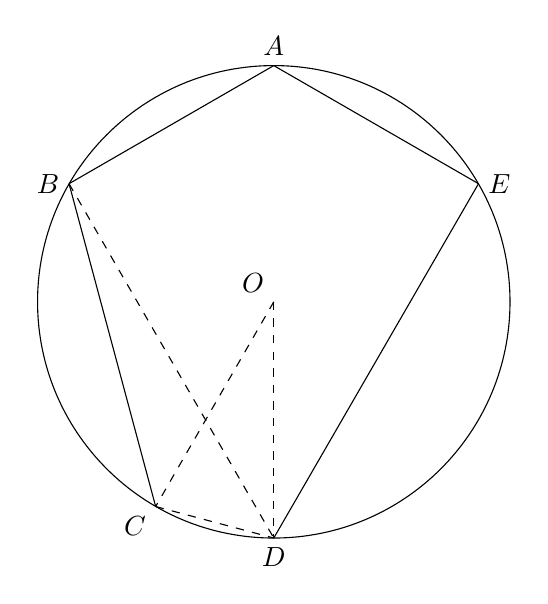
\begin{tikzpicture}
  \coordinate (O) at (0,0);
  \coordinate (A) at (0,3);
  \coordinate (B) at (-2.6,1.5);
  \coordinate (C) at (-1.5,-2.6);
  \coordinate (D) at (0,-3);
  \coordinate (E) at (2.6,1.5);

  \draw (0,0) circle (3);

  \draw (A) -- (B);
  \draw (A) -- (E);
  \draw (B) -- (C);
  \draw (E) -- (D);

  \draw[dashed] (O) -- (C);
  \draw[dashed] (O) -- (D);
  \draw[dashed] (B) -- (D);
  \draw[dashed] (C) -- (D);

  \node[above] at (A) {$A$};
  \node[left] at (B) {$B$};
  \node[below left] at (C) {$C$};
  \node[below] at (D) {$D$};
  \node[right] at (E) {$E$};
  \node[above left] at (O) {$O$};
\end{tikzpicture}
\end{document}
